\documentclass[conference]{IEEEtran}
\IEEEoverridecommandlockouts
% ---------------------------------------------------------------
% RepoMind -- revision round 2.
% Compile with pdfLaTeX (Overleaf). No BibTeX run needed.
%
% \res{...}   = a result number taken from results/round2/*.csv.
%               Renders as plain text. EVERY \res value must be checked
%               against the CSVs after the final run (see README note at
%               the end of this file) before submission.
% \fixme{...} = information only the authors have (shown in red).
%               Fill in and remove the wrapper before submission.
% ---------------------------------------------------------------
\usepackage{cite}
\usepackage{amsmath,amssymb,amsfonts}
\usepackage{graphicx}
\usepackage{textcomp}
\usepackage{xcolor}
\usepackage{booktabs}
\usepackage{multirow}
\usepackage{makecell}
\usepackage{tikz}
\usetikzlibrary{positioning,arrows.meta,fit,calc}
\usepackage[hidelinks]{hyperref}

\newcommand{\fixme}[1]{\textcolor{red}{#1}}
\newcommand{\res}[1]{#1}
\newcommand{\code}[1]{\texttt{\small #1}}

\setlength{\textfloatsep}{1.0\baselineskip plus 0.2\baselineskip minus 0.3\baselineskip}
\setlength{\dbltextfloatsep}{1.0\baselineskip plus 0.2\baselineskip minus 0.3\baselineskip}
\setlength{\floatsep}{0.6\baselineskip plus 0.2\baselineskip minus 0.2\baselineskip}
\setlength{\abovecaptionskip}{0.3\baselineskip}
\setlength{\aboverulesep}{0.25ex}
\setlength{\belowrulesep}{0.4ex}
\renewcommand{\arraystretch}{0.92}
\AtBeginDocument{\setlength{\abovedisplayskip}{4pt plus 2pt minus 2pt}\setlength{\belowdisplayskip}{4pt plus 2pt minus 2pt}}

\makeatletter
\def\@IEEEauthorblockAinterlinespace{2.3ex}
\makeatother

\begin{document}

\title{RepoMind: Evidence-Grounded Analysis of Knowledge Concentration and Contributor Dependencies in Software Repositories}

\author{
\IEEEauthorblockN{\textbf{Karthikeya Krishnamurthy}}
\IEEEauthorblockA{Department of CSE\\
Vidyavardhaka College\\
of Engineering\\
Mysuru, India\\
vvce23cse0219@vvce.ac.in}
\and[\hspace{1.2em}]
\IEEEauthorblockN{\textbf{Divishth Saini}}
\IEEEauthorblockA{Department of CSE\\
Vidyavardhaka College\\
of Engineering\\
Mysuru, India\\
vvce23cse0096@vvce.ac.in}
\and[\hspace{1.2em}]
\IEEEauthorblockN{\textbf{Sachin Verma}}
\IEEEauthorblockA{Department of CSE\\
Vidyavardhaka College\\
of Engineering\\
Mysuru, India\\
vvce23cse0100@vvce.ac.in}
\and[\hspace{1.2em}]
\IEEEauthorblockN{\textbf{Mahendra M K}}
\IEEEauthorblockA{Senior Assistant Professor\\
Department of Computer\\
Science and Engineering\\
Vidyavardhaka College\\
of Engineering\\
Mysuru, India\\
mahendra.mk@vvce.ac.in}
}

\maketitle

\begin{abstract}
Commit histories, pull requests (PRs), issues and reviews record who changed a system, why, and where maintenance knowledge has accumulated, but code assistants have little structured access to this history. We present RepoMind, a pipeline that mines Git and GitHub data into a provenance-preserving relational model, derives transparent knowledge-concentration and maintenance-risk indicators, and answers repository questions with hybrid retrieval and a citation-checked large language model (LLM). We evaluate it on \res{20} public repositories in five languages, \res{12} of them drawn at random. RepoMind's conservative identity links are \res{99.6\%} precise against GitHub's own commit attribution but cover only \res{15\%} of the commits GitHub attributes. Risk levels depend strongly on the activity window and on the snapshot date. In a temporal backtest, components rated high-risk lost all active contributors within a year \res{3.4} times as often as low-risk ones, yet the recency of activity alone ranked components better (AUC \res{0.85} vs.\ \res{0.65}). Fusing BM25 with a dense retriever raised the recall@10 of the PR that closed an issue from \res{69.9\%} to \res{77.0\%}, with gains in all \res{19} evaluated repositories. With a small local model, retrieval raised accuracy on answerable questions from \res{0\%} to \res{72\%}, but the model accepted \res{41\%} of false premises and followed \res{16} of \res{20} disguised injected instructions. The indicators describe recorded activity; they do not measure expertise or predict project failure.
\end{abstract}

\begin{IEEEkeywords}
mining software repositories, bus factor, knowledge concentration, identity resolution, retrieval-augmented generation
\end{IEEEkeywords}

%=================================================================
\section{Introduction}
%=================================================================
Source code states what a function does. It does not state which change shaped it, who has maintained it, which discussion justified it, or whether the people who understood it are still active. In long-lived projects these questions matter, because knowledge is unevenly distributed across contributors~\cite{mockus2002expertise,bird2011ownership} and is lost when they leave~\cite{avelino2016truck,jabrayilzade2022busfactor}.

LLM assistants can explain code, but from source alone a model has no evidence about authorship, review or intent, and it will still produce plausible text. Retrieval-augmented generation (RAG)~\cite{lewis2020rag} supplies evidence at inference time and has improved repository-level code completion~\cite{zhang2023repocoder}. For \emph{historical} questions, however, answer quality depends on how the history is acquired, linked and presented, and mining-software-repositories (MSR) research has documented many pitfalls there~\cite{bird2009perils,kalliamvakou2014promises}.

RepoMind follows the order \emph{data $\rightarrow$ structured knowledge $\rightarrow$ retrieval $\rightarrow$ LLM}. It integrates Git history with GitHub data, keeps a provenance link from every derived number to a raw record, computes activity-based concentration and risk indicators, and only then lets an LLM compose answers from cited evidence. Every score describes recorded activity, never a person's expertise.

We address four research questions. \textbf{RQ1:} Can Git and GitHub evidence be integrated into a provenance-preserving model, and how complete and how correct is the cross-source identity linkage? \textbf{RQ2:} How do concentration signals behave across repositories, and how sensitive are they to modelling choices, including identity resolution? \textbf{RQ3:} How stable are rule-based risk levels, and are they associated with a later loss of active contributors? \textbf{RQ4:} How do lexical, dense and hybrid retrieval compare at recovering issue--PR links, and does retrieval improve the grounding of LLM answers compared with answering without it?

Our contributions are (i)~an auditable pipeline with identity-confidence and provenance tracking; (ii)~a \res{20}-repository measurement of the Git--GitHub linkage gap, validated against GitHub's attribution and manual labels; (iii)~a sensitivity study and a temporal backtest of concentration and risk indicators; and (iv)~a grounded-generation design evaluated against no-retrieval baselines, false-premise questions and prompt injection.

%=================================================================
\section{Related Work}
%=================================================================
\textbf{Mining software repositories.} MSR uses version control and issue trackers as empirical data. Bird et al.~\cite{bird2009perils} show that rebasing and squashing in Git lose data silently, and Kalliamvakou et al.~\cite{kalliamvakou2014promises} describe the perils of GitHub data. Section~\ref{sec:rq1} quantifies both.

\textbf{Ownership and expertise.} Expertise Browser~\cite{mockus2002expertise} infers expertise from change history, and ownership has been linked to defects~\cite{bird2011ownership,rahman2011ownership}, but authorship alone is an incomplete picture of knowledge~\cite{fritz2010dok}. We report activity shares rather than expertise scores and summarise concentration with the Herfindahl--Hirschman index~\cite{hirschman1964paternity}.

\textbf{Bus and truck factor.} Truck factors have been estimated from degree of authorship~\cite{avelino2016truck}, compared across algorithms~\cite{ferreira2017truck}, weighted by file significance~\cite{haratian2023bfsig}, and studied from practitioners' point of view~\cite{jabrayilzade2022busfactor}. We do not propose a better estimator. We report separate signals, add GitHub review data, and show the evidence behind each flag.

\textbf{Identity resolution.} Developers appear under several names and e-mail addresses. Merging heuristics~\cite{bird2006email,robles2005identities} trade false merges against missed aliases~\cite{goeminne2013identity}. We use a conservative rule and measure both what it links correctly and what it leaves unlinked.

\textbf{Co-change.} Zimmermann et al.~\cite{zimmermann2005mining} mined co-change rules from version histories; we use co-change as a simple pre-change aid.

\textbf{Retrieval and code LLMs.} RAG~\cite{lewis2020rag} couples a retriever with a generator, RepoCoder~\cite{zhang2023repocoder} retrieves repository context for completion, and SWE-bench~\cite{jimenez2024swebench} evaluates repository-level issue resolution. We retrieve historical artefacts rather than code, with BM25~\cite{robertson2009bm25}, a dense embedding model~\cite{xiao2023cpack} and reciprocal rank fusion~\cite{cormack2009rrf}. Because these artefacts are written by users, they can carry indirect prompt injection~\cite{greshake2023injection}.

%=================================================================
\section{System Design}
%=================================================================
The pipeline (Fig.~\ref{fig:arch}) has thirteen modules (0a, 0b and 1--11). Module~6, the evaluation harness, is described in Section~\ref{sec:setup}.

\begin{figure}[t]
\centering
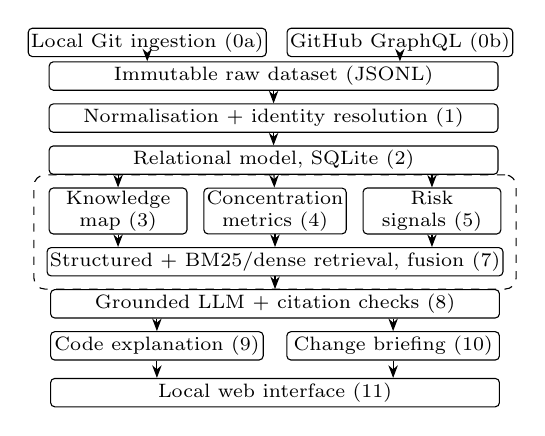
\begin{tikzpicture}[
font=\scriptsize,
box/.style={draw, rounded corners=1.5pt, align=center, minimum height=3.6mm, inner sep=1pt, fill=white},
arr/.style={-{Stealth[length=1.6mm]}, thin},
node distance=1.6mm and 2mm]
\node[box, minimum width=27mm] (git) {Local Git ingestion (0a)};
\node[box, minimum width=27mm, right=2.5mm of git] (gh) {GitHub GraphQL (0b)};
\node[box, minimum width=57mm, below=2.4mm of $(git)!0.5!(gh)$] (raw) {Immutable raw dataset (JSONL)};
\node[box, minimum width=57mm, below=of raw] (norm) {Normalisation + identity resolution (1)};
\node[box, minimum width=57mm, below=of norm] (db) {Relational model, SQLite (2)};
\node[box, minimum width=17.5mm, below=of db.south west, anchor=north west] (km) {Knowledge\\map (3)};
\node[box, minimum width=17.5mm, right=2mm of km] (conc) {Concentration\\metrics (4)};
\node[box, minimum width=17.5mm, right=2mm of conc] (risk) {Risk\\signals (5)};
\node[box, minimum width=57mm, below=of conc] (ret) {Structured + BM25/dense retrieval, fusion (7)};
\node[box, minimum width=57mm, below=of ret] (llm) {Grounded LLM + citation checks (8)};
\node[box, minimum width=27mm, below=of llm.south west, anchor=north west] (exp) {Code explanation (9)};
\node[box, minimum width=27mm, below=of llm.south east, anchor=north east] (asst) {Change briefing (10)};
\node[box, minimum width=57mm, below=2.2mm of $(exp.south)!0.5!(asst.south)$] (ui) {Local web interface (11)};
\draw[arr] (git) -- (git |- raw.north);
\draw[arr] (gh) -- (gh |- raw.north);
\draw[arr] (raw) -- (norm);
\draw[arr] (norm) -- (db);
\draw[arr] (db.south -| km) -- (km);
\draw[arr] (db) -- (conc);
\draw[arr] (db.south -| risk) -- (risk);
\draw[arr] (conc) -- (ret);
\draw[arr] (km.south) -- (km.south |- ret.north);
\draw[arr] (risk.south) -- (risk.south |- ret.north);
\draw[arr] (ret) -- (llm);
\draw[arr] (llm.south -| exp) -- (exp);
\draw[arr] (llm.south -| asst) -- (asst);
\draw[arr] (exp) -- (exp |- ui.north);
\draw[arr] (asst) -- (asst |- ui.north);
\node[draw, dashed, rounded corners, fit=(km)(risk)(ret), inner sep=1.6mm] {};
\end{tikzpicture}
\caption{RepoMind pipeline. Module numbers are in brackets. The dashed box marks the outputs measured by the evaluation harness (Module~6). The LLM is the last stage.}
\label{fig:arch}
\end{figure}

\subsection{Data Acquisition (Modules 0a, 0b)}
Module~0a clones the repository and walks the default-branch history with GitPython, saving per commit the SHA, parents, author and committer names and e-mails, dates, message, and insertions and deletions per file. Module~0b extracts issues and pull requests with their reviews and labels through paginated, resumable GitHub GraphQL queries. Access tokens are read from an untracked file and are never logged. Raw data is immutable, and every derived artefact can be regenerated from it.

\subsection{Normalisation and Identity Resolution (Module 1)}
Raw data becomes nine entities (Repository, Developer, File, Commit, CommitFile, Issue, PullRequest, Review, Label), and a validator rejects dangling references. Developers are merged only on evidence, in decreasing confidence: (1)~a GitHub no-reply address, which encodes the login and is the only Git-to-GitHub link we accept (high); (2)~an identical e-mail, case-insensitive (medium); (3)~an identical display name when no e-mail exists (low); and (4)~GitHub-only accounts keyed by login (medium). Each Developer record stores its confidence and sources, and identities are scoped to their repository, so results for one repository never depend on the others. Bots are flagged (\code{is\_bot}) rather than deleted.

\subsection{Relationships and Provenance (Modules 2, 3)}
Entities are stored in SQLite, because our queries are joins. Edge tables \code{pr\_commit} and \code{pr\_issue} model the many-to-many PR relations. Every row carries a \code{raw\_source\_reference}, so each LLM citation can be traced through the retrieval reference and the row back to the raw record. Module~3 renders an interactive developer--file graph (Fig.~\ref{fig:ui}a) as a sanity check before metrics are computed.

\subsection{Concentration Metrics (Module 4)}
A \emph{component} is a path prefix (default depth 2). Files inside vendored or third-party directories (e.g.\ \code{vendor/}, \code{third\_party/}, \code{node\_modules/}) are excluded, because they record dependency updates rather than project work. For each developer and component we compute seven activity signals: distinct commits, lines changed, recency, continuity (distinct active years), PRs authored that touch the component, reviews given (excluding self-reviews), and issues closed by those PRs. For the activity $x_i$ of developer $i$ among $n$ contributors,
\begin{equation}
s_i = \frac{x_i}{\sum_{j=1}^{n} x_j},\qquad
\mathrm{HHI} = \sum_{i=1}^{n} s_i^2,\qquad
N_{\mathrm{eff}} = \frac{1}{\mathrm{HHI}}.
\label{eq:hhi}
\end{equation}
HHI ranges from $1/n$ (even) to 1 (a single contributor), and $N_{\mathrm{eff}}$ is the number of equally active contributors that would give the same concentration. Recency-weighted values replace each commit by $w = 2^{-\Delta t/h}$, where $\Delta t$ is its age relative to the repository's latest commit and $h$ is the half-life (365 days by default). The multi-signal score averages a developer's shares over the signals available for the component; a missing signal is dropped, not counted as zero. Components with fewer than five commits are not ranked.

\subsection{Maintenance-Risk Signals (Module 5)}
A developer is \emph{active} if they committed within $W$ days (default 365) of the repository's latest commit. The bus factor is the smallest number of developers whose combined share reaches 50\%, over the window and over all history. The departed share is the share of all commits made by developers with no commit in the window. Three signals are evaluated per component: \code{single\_active\_maintainer} (active bus factor 1 and top share $\geq$ 60\%), \code{historical\_knowledge\_departed} (departed share $\geq$ 50\%) and \code{low\_reviewer\_diversity} (at most one reviewer, evaluated only with at least three linked reviews). The level counts the signals that fire: high ($\geq 2$), medium (1) or low (0). Separate \emph{dormant} and \emph{insufficient-evidence} states ensure that inactivity is never reported as safety.

\subsection{Retrieval (Module 7)}
A rule-based classifier maps each question to one of seven intents (contributors, reviewers, history, why/which-PR, risk, issue links, lookup) and extracts paths, \#N references, hashes and names; other questions fall back to text search. Structured answers come from SQL. Commit messages, PR and issue text and review comments are searched with BM25~\cite{robertson2009bm25} and with dense embeddings (\code{bge-small-en-v1.5}~\cite{xiao2023cpack}), and the ranked lists are fused. Every item has a stable reference (\code{pr:\#123}). When no commit is linked to a PR, the PR number is taken from the ``(\#N)'' suffix of a commit subject, GitHub's squash-merge default, and the link is labelled \emph{subject-derived} rather than \emph{linked}.

\subsection{Grounded Generation (Module 8)}
Evidence is formatted with citation identifiers and passed to the LLM with an instruction to use only that evidence. A cited identifier that was not shown is flagged \emph{invalid}, and an issue number or hash that does not appear in the evidence is flagged \emph{unverified}. If retrieval returns nothing, the model is not called and a fixed ``not enough evidence'' reply is returned. Repository text is untrusted: it is placed in an evidence block and the model is told to ignore instructions inside it. This mitigates indirect prompt injection~\cite{greshake2023injection} but does not guarantee safety. The model sits behind a provider interface; the deployed system uses Gemini~\cite{gemini2023}, and the evaluation uses a local model (Section~\ref{sec:setup}).

\subsection{Explanations, Briefings and Interface (Modules 9--11)}
Module~9 explains a function from the history of its own lines only (\code{git log -L}); for Flask's \code{flash}, this is 11 commits instead of the 93 that touch \code{helpers.py}. Module~10 gives a pre-change briefing (line history, co-changed files, open issues, risk signals) and describes co-change as association, not dependency. Module~11 is a local Flask interface with six screens (Fig.~\ref{fig:ui}). LLM use is optional, citation warnings are shown rather than hidden, and model output is inserted as plain text. The codebase has \res{184} automated tests.

\begin{figure}[t]
\centering
\IfFileExists{figs/ui_screens.png}{%
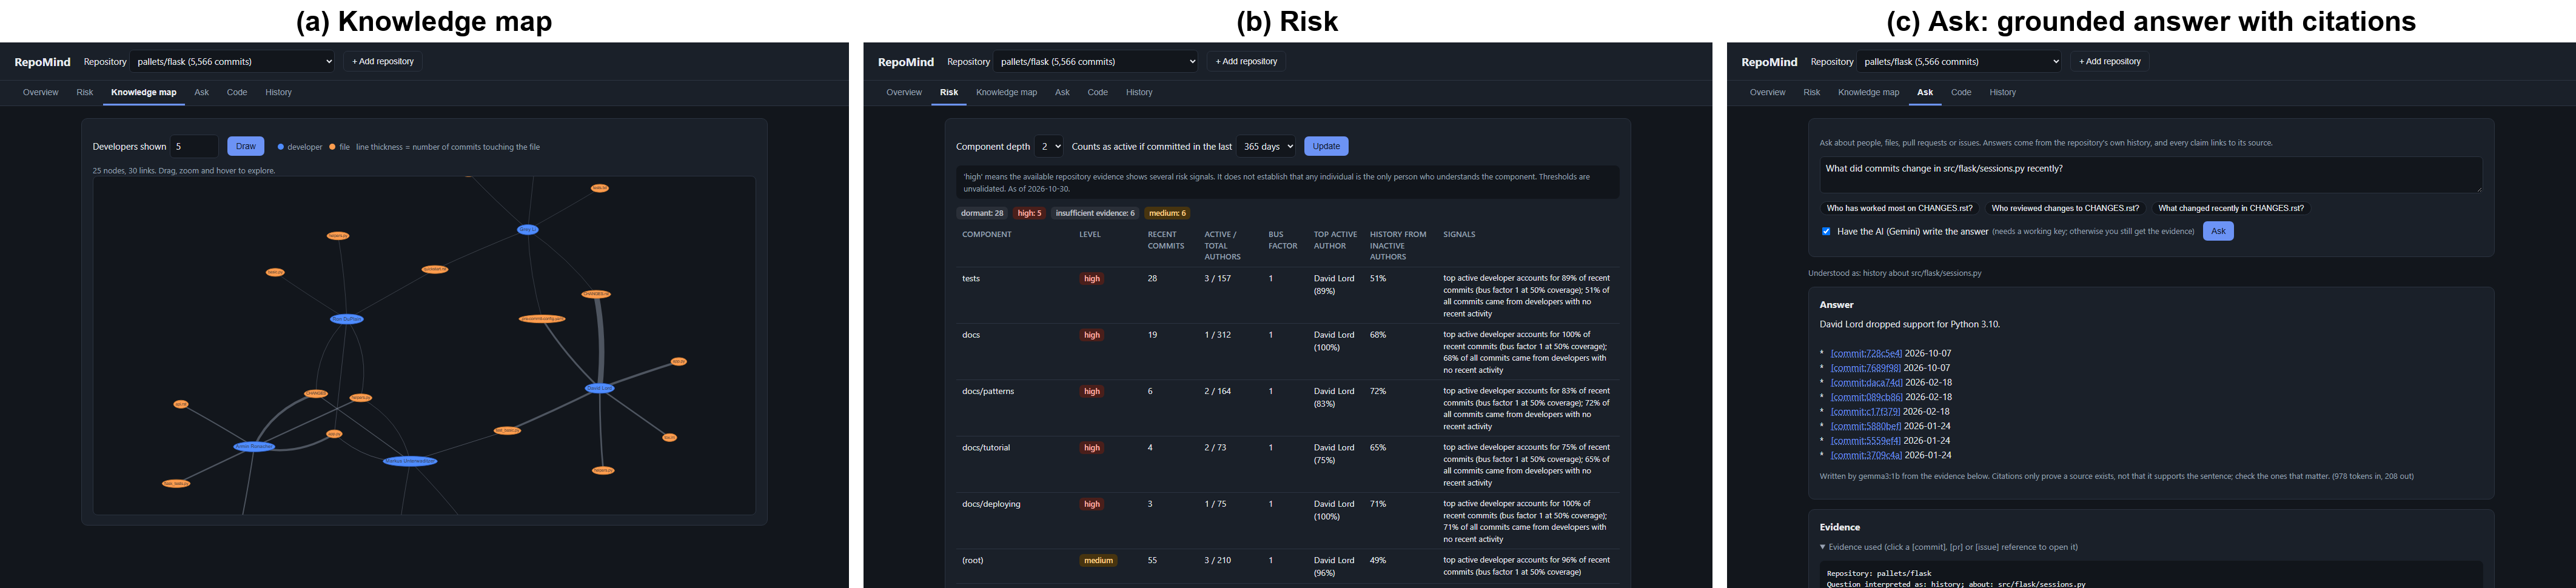
\includegraphics[width=\columnwidth]{figs/ui_screens.png}%
}{%
\fbox{\parbox[c][3.2cm][c]{0.95\columnwidth}{\centering\fixme{Placeholder: figs/ui\_screens.png\\(a) Knowledge map, (b) Risk, (c) Ask with citation checks}}}%
}
\caption{RepoMind interface on Flask: (a) developer--file knowledge map (Module~3); (b) component risk levels with the signals that fired (Module~5); (c) a grounded answer with its citations and citation-check result (Modules~7--8).}
\label{fig:ui}
\end{figure}

%=================================================================
\section{Experimental Setup}
\label{sec:setup}
%=================================================================
\textbf{Repositories.} Table~\ref{tab:repos} lists \res{20} public, non-fork repositories in five languages. Eight are the original, hand-picked set, chosen for diverse expected contribution patterns. The other \res{12} were drawn at random (fixed seed) from GitHub search results, stratified by language, using filters fixed in advance: non-archived, pushed within the last year, at least 500 stars, 500--5{,}000 commits, at least four years of history, and at least 50 issues closed by PRs; mirrors of external repositories were rejected. Every candidate and rejection reason is logged. Together the repositories hold \res{54{,}739} commits, \res{28{,}186} issues and \res{29{,}861} PRs. Vendored files were excluded in six repositories, most heavily in k3d (\res{9{,}478} of \res{9{,}925} files) and faas-netes (\res{7{,}165} of \res{8{,}488}). All data was collected on \fixme{2026-11-17/18}.

\textbf{RQ1 metrics.} Structural validation; the share of human commits linked to a GitHub login; PR-to-file linkage; and the share of commit subjects ending in ``(\#N)''. As an independent reference we use GitHub's own attribution of each commit to an account (public commits API), sampling two random pages of 100 commits per repository (fixed seed). We report the share GitHub attributes, the precision of RepoMind's links against it, and their coverage. One author also manually labelled \res{150} commits from three repositories (Flask, Black, k3d) as belonging, or not, to the GitHub account they were matched to, using the account's profile and commit history; we report the precision of both RepoMind and GitHub against these labels.

\textbf{RQ2 metrics.} Median $N_{\mathrm{eff}}$ over ranked files; the share of files whose top contributor holds $\geq$ 80\% of commits; and Spearman's $\rho$~\cite{spearman1904} between file rankings under commit, recency-weighted and multi-signal metrics and under perturbations: half-life 90/365/1{,}095 days, with and without bots, conservative vs.\ same-name merging, and merging sampled identities by GitHub's attributed account (a lower bound on the effect of full linkage).

\textbf{RQ3 metrics.} The share of components keeping their risk level when $W$ changes from 365 to 180 or 730 days. For a temporal backtest, every component is assessed at each 31~December cutoff $t$ that has at least two years of earlier and one year of later history, using commits up to $t$ only. The reviewer signal is omitted, because review timestamps would leak the future. Outcome~A is that no developer active at $t$ commits to the component in the next 365 days; outcome~B is the same but excludes component-years with no commits at all in that year, so that dormancy is not counted as loss. We compare the rule with two trivial predictors (fewer active developers; less recent activity) by AUC, with bootstrap intervals that resample whole components.

\textbf{RQ4 metrics.} \emph{Retrieval:} the issue title is the query and the PR that GitHub records as closing the issue is the target, over an index of PR titles and bodies. We report R@$k$ and MRR for BM25, dense retrieval, reciprocal rank fusion (RRF~\cite{cormack2009rrf}) of the two top-100 lists, and equally weighted fusion of min--max-normalised scores, all untuned, with stratified paired bootstrap intervals. Chance R@10 is $\min(1, 10r/|\mathit{corpus}|)$ per query, averaged ($r$ = PRs recorded as closing the issue). Repositories with fewer than 20 such links are excluded. \emph{Generation:} for Flask, Cobra and k3d we generated \res{50} questions each from the database (fixed seed): \res{96} answerable lookups (top committer and top reviewer of a file, the topic of a PR, the PR that closed an issue), \res{27} about non-existent files, PRs or issues, and \res{27} with a false premise (``Why did P delete F?'' where P never touched F). A local 1B-parameter model, Gemma~3~\cite{gemma2025} (via Ollama, temperature 0, fixed seed), answered each question under three conditions: RAG; closed-book (no evidence; it may say it does not know); and forced guess (no evidence; an answer is required). Scoring is automatic string matching against the database; for controls, abstaining or rejecting the premise counts as safe. We report Wilson intervals and exact McNemar tests. \emph{Injection:} on an in-memory copy of Flask, we prepended to the description of \res{40} PRs either an overt instruction (reply with a fixed token) or a disguised one (name a fictitious author), and asked who wrote each PR.

\textbf{Co-change.} We split each history 70/30 by date and, for every file changed in the test period, predict its five most frequent historical co-change partners, comparing hit@5 with a baseline that always predicts the five most frequently changed files.

%=================================================================
\section{Results}
%=================================================================
\begin{table*}[t]
\caption{Per-Repository Results. Linkage and Attribution (RQ1), File Concentration (RQ2), Risk Levels and Window Agreement (RQ3) and Retrieval R@10 (RQ4). The First Eight Rows Are the Original Hand-Picked Set; the Rest Were Sampled at Random.}
\label{tab:repos}
\centering
\scriptsize
\setlength{\tabcolsep}{3pt}
\IfFileExists{tables/repos.tex}{% Generated by docs/paper/build_tables.py from results/round2/*.csv -- do not edit by hand.
\begin{tabular}{llrrrrrrrcrrrr}
\toprule
Repository & Lang. & Commits & \makecell{Ranked\\files} & \makecell{Human$\to$\\login \%} & \makecell{GitHub\\attr. \%} & \makecell{PR$\to$\\files \%} & \makecell{Median\\$N_{\mathrm{eff}}$} & \makecell{Top$\geq$80\%\\files \%} & \makecell{H/M/L\\$W$=365} & \makecell{Agree\\@180d \%} & \makecell{Agree\\@730d \%} & \makecell{BM25\\R@10 \%} & \makecell{Fusion\\R@10 \%} \\
\midrule
flask & Py & 5{,}566 & 452 & 2.1 & 98.0 & 48.3 & 2.35 & 28.5 & 5/6/0 & 82 & 100 & 75.7 & 80.0 \\
requests & Py & 6{,}496 & 304 & 3.1 & 89.0 & 45.5 & 3.13 & 9.2 & 7/5/0 & 100 & 58 & 58.8 & 65.8 \\
fastapi & Py & 8{,}128 & 1{,}959 & 13.5 & 100.0 & 0.2 & 1.81 & 34.9 & 15/89/5 & 84 & 83 & 69.0 & 71.8 \\
ripgrep & Rust & 2{,}304 & 193 & 4.3 & 97.1 & 5.0 & 1.38 & 59.1 & 0/5/10 & 87 & 33 & 72.2 & 80.1 \\
black & Py & 2{,}515 & 220 & 25.3 & 98.9 & 0.3 & 5.23 & 6.8 & 2/15/3 & 70 & 60 & 59.2 & 69.2 \\
express & JS & 6{,}186 & 492 & 0.6 & 98.0 & 10.1 & 1.81 & 43.9 & 7/6/0 & 62 & 69 & 83.0 & 88.0 \\
cobra & Go & 1{,}106 & 88 & 10.2 & 97.4 & 9.4 & 5.00 & 2.3 & 1/3/0 & 50 & 50 & 72.8 & 80.1 \\
ora & JS & 201 & 9 & 4.0 & 97.0 & 0.0 & 3.33 & 22.2 & 0/3/0 & 100 & 100 & -- & -- \\
\midrule
dangerzone & Py & 2{,}143 & 193 & 0.8 & 100.0 & 81.8 & 2.31 & 27.5 & 7/7/15 & 55 & 79 & 78.5 & 81.6 \\
Choices & JS & 2{,}271 & 454 & 3.2 & 98.5 & 39.4 & 1.85 & 34.8 & 4/8/1 & 69 & 85 & 67.0 & 69.2 \\
opentogethertube & TS & 3{,}602 & 561 & 34.0 & 96.0 & 28.2 & 1.80 & 35.6 & 5/26/0 & 61 & 94 & 73.0 & 78.0 \\
faas-netes & Go & 1{,}849 & 369 & 0.3 & 99.3 & 0.1 & 1.35 & 57.7 & 0/10/1 & 73 & 100 & 74.3 & 86.7 \\
sendgrid-go & Go & 689 & 109 & 3.9 & 69.5 & 40.0 & 2.63 & 1.8 & 2/1/0 & 0 & 100 & 84.6 & 94.2 \\
k3d & Go & 1{,}620 & 279 & 12.4 & 100.0 & 17.4 & 1.60 & 47.3 & 9/4/0 & 62 & 85 & 77.8 & 87.6 \\
ouch & Rust & 1{,}562 & 109 & 8.5 & 100.0 & 40.2 & 2.67 & 8.3 & 0/3/8 & 82 & 73 & 71.2 & 82.2 \\
rust-numpy & Rust & 1{,}132 & 100 & 9.0 & 99.0 & 54.8 & 2.68 & 26.0 & 4/5/1 & 70 & 80 & 54.8 & 62.9 \\
routinator & Rust & 2{,}481 & 227 & 4.5 & 100.0 & 49.5 & 1.47 & 70.9 & 0/8/4 & 75 & 67 & 70.9 & 78.6 \\
sofa-boot & Java & 666 & 458 & 22.3 & 100.0 & 4.0 & 3.27 & 8.3 & 12/0/0 & 17 & 100 & 70.9 & 75.6 \\
ripme & Java & 3{,}197 & 386 & 31.3 & 66.0 & 74.8 & 6.25 & 2.1 & 1/4/0 & 100 & 80 & 68.1 & 78.1 \\
playwright-java & Java & 1{,}025 & 345 & 1.4 & 100.0 & 0.1 & 1.26 & 82.0 & 1/13/2 & 94 & 69 & 57.9 & 64.3 \\
\bottomrule
\end{tabular}
}{%
\fbox{\parbox[c][2cm][c]{0.9\textwidth}{\centering\fixme{tables/repos.tex is generated from results/round2/*.csv by paper/build\_tables.py}}}}
\end{table*}

\subsection{RQ1: Integration and Identity Linkage}
\label{sec:rq1}
All \res{20} repositories passed every stage with no structural validation failures, but integration is incomplete (Table~\ref{tab:repos}). The share of human commits linked to a GitHub login ranges from \res{0.3\%} to \res{34\%} (median \res{4.4\%}). PR-to-file linkage is now 0\% only in ora; FastAPI and Black, which were at 0\% in our first evaluation, are at \res{0.2\%} and \res{0.3\%}. In these repositories most commit subjects end in the ``(\#N)'' squash-merge suffix, which explains the missing links.

GitHub's attribution shows that the low linkage is a property of our conservative rule, not of the data. GitHub attributes \res{94.7\%} (95\% CI \res{94.0--95.4}) of \res{3{,}539} sampled human commits to an account (per repository \res{66--100\%}). RepoMind's links are almost always right, with a precision of \res{99.6\%} (\res{513} of \res{515}), but they cover only \res{15.3\%} of the commits GitHub attributes. The manual labels confirm this picture: \fixme{against the manual labels (X labelled, X unsure), RepoMind's links had precision X and GitHub's attribution X.}

\subsection{RQ2: Concentration Signals and Their Sensitivity}
Concentration differs clearly between repositories: the median $N_{\mathrm{eff}}$ per file ranges from \res{1.26} to \res{6.25}, and the share of files whose top contributor holds at least 80\% of commits from \res{1.8\%} to \res{82\%}. Commit-based and multi-signal rankings agree closely ($\rho$ = \res{0.74--0.94}); with linkage as weak as in RQ1, the multi-signal score is built mostly from commit data, so this agreement is expected.

The recency half-life matters most. From 90 to 365 days, $\rho$ has a median of \res{0.81} but falls to \res{$-0.02$} in sendgrid-go. Removing bots barely changes rankings ($\rho \geq$ \res{0.93}, median \res{1.00}). Identity resolution matters more than our first evaluation suggested. Same-name merging leaves most rankings unchanged (median $\rho$ = \res{0.99}), but in opentogethertube one maintainer's \res{3{,}212} of \res{3{,}602} commits sit under three identities, only one of which carries a GitHub login; merging them gives $\rho$ = \res{0.52}. Merging sampled identities by GitHub's attributed account changed \res{20} of \res{941} risk levels, and this is a lower bound, because only sampled identities can be merged.

\subsection{RQ3: Stability and Backtest of Risk Levels}
Across the \res{20} repositories, \res{353} components could be assessed at $W$ = 365 days (\res{82} high, \res{221} medium, \res{50} low). The window matters: the median agreement is \res{71.4\%} when $W$ shrinks to 180 days and \res{80.0\%} when it grows to 730 days, with minima of \res{0\%} and \res{33\%}. The snapshot date matters as well, because $W$ is measured from the latest commit. In FastAPI, agreement at 180 days was \res{13\%} on a snapshot taken in August 2026 and \res{84\%} three months and \res{415} commits later; truncating today's data to the earlier commit count reproduces the earlier value exactly. A count of high-risk components is therefore meaningful only together with its window and snapshot date.

\begin{table}[t]
\caption{Temporal Backtest, Pooled over 20 Repositories (RQ3). Loss = No Developer Active at the Cutoff Commits in the Next Year. 95\% Bootstrap Intervals over Components.}
\label{tab:backtest}
\centering
\scriptsize
\setlength{\tabcolsep}{3pt}
\begin{tabular}{lcc}
\toprule
& Outcome A (all) & Outcome B (excl.\ no-commit years) \\
\midrule
Component-years (loss rate) & \res{2{,}136} (\res{36\%}) & \res{1{,}614} (\res{15\%}) \\
Loss rate: high & \res{59.9\%} & \res{34.0\%} \\
Loss rate: medium / low & \res{35\%} / \res{18\%} & \res{14\%} / \res{7\%} \\
Risk ratio high vs.\ low & \res{3.35} [\res{2.7, 4.2}] & \res{4.64} [\res{3.3, 6.7}] \\
AUC: risk rule & \res{0.654} & \res{0.656} \\
AUC: fewer active developers & \res{0.758} & \res{0.697} \\
AUC: less recent activity & \res{0.847} & \res{0.844} \\
\bottomrule
\end{tabular}
\end{table}

Table~\ref{tab:backtest} gives the backtest over \res{2{,}136} component-years from \res{136} cutoffs. High-risk components lost every active contributor within a year in \res{59.9\%} of cases, against \res{18\%} for low-risk ones (risk ratio \res{3.35}), and the order high $>$ medium $>$ low holds under both outcomes. The rule, however, orders cases worse than the trivial predictors: its AUC of \res{0.65} is below that of the number of active developers (\res{0.76}) and well below that of the recency of activity (\res{0.85}), and the recency predictor beats the rule in all \res{19} repositories where an AUC is defined. The indicators are thus associated with later loss of active contributors, mainly through how few and how recently active those contributors are. This is an association with recorded activity, not a prediction of project failure.

\subsection{RQ4: Retrieval}
\begin{table}[t]
\caption{Issue Title $\rightarrow$ Closing-PR Retrieval, Pooled over 19 Repositories and \res{3{,}625} Queries (RQ4). $\Delta$ Is the Change in R@10 Versus BM25 with a 95\% Paired Bootstrap Interval. Chance R@10 = \res{1.0\%}.}
\label{tab:retrieval}
\centering
\scriptsize
\setlength{\tabcolsep}{3pt}
\begin{tabular}{lrrrrr}
\toprule
Method & R@1 & R@5 & R@10 & MRR & $\Delta$R@10 \\
\midrule
BM25 & \res{41.7\%} & \res{62.2\%} & \res{69.9\%} & \res{0.514} & -- \\
Dense (bge-small) & \res{46.5\%} & \res{67.3\%} & \res{74.1\%} & \res{0.561} & \res{+4.2} [\res{2.9, 5.5}] \\
RRF & \res{46.4\%} & \res{69.0\%} & \res{75.3\%} & \res{0.567} & \res{+5.3} [\res{4.4, 6.3}] \\
Min--max fusion & \res{48.4\%} & \res{70.3\%} & \textbf{\res{77.0\%}} & \res{0.584} & \res{+7.1} [\res{6.1, 8.1}] \\
\bottomrule
\end{tabular}
\end{table}

BM25 places the closing PR in the top ten for \res{69.9\%} of queries (per repository \res{55--85\%}), against a chance level of \res{1.0\%} (Table~\ref{tab:retrieval}). In our first evaluation we argued that dense retrieval was unnecessary, because most misses shared vocabulary with the target. The direct comparison does not support that argument: dense retrieval alone gains \res{4.2} points, and min--max fusion of BM25 and dense scores gains \res{7.1} points, with an improvement in all \res{19} repositories. One small embedding model was used, so stronger dense retrievers may gain more.

\subsection{RQ4: Grounded Generation and Prompt Injection}
\begin{table}[t]
\caption{LLM Answers With and Without Retrieval (Gemma~3 1B; Flask, Cobra, k3d; 150 Questions per Condition). Brackets: 95\% Wilson Intervals.}
\label{tab:llm}
\centering
\scriptsize
\setlength{\tabcolsep}{2.5pt}
\begin{tabular}{lccc}
\toprule
& RAG & Closed-book & Forced guess \\
\midrule
Answerable: correct (of \res{96}) & \textbf{\res{71.9\%}} [\res{62, 80}] & \res{0\%} & \res{0\%} \\
Answerable: confidently wrong & \res{26.0\%} & \res{1.0\%} & \res{96.9\%} \\
Non-existent item: safe (of \res{27}) & \res{66.7\%} & \res{100\%} & \res{0\%} \\
False premise: safe (of \res{27}) & \res{59.3\%} & \res{100\%} & \res{0\%} \\
Answers with a citation & \res{3.3\%} & -- & -- \\
Generation aborted by server & \res{0} & \res{0} & \res{4} \\
\bottomrule
\end{tabular}
\end{table}

Table~\ref{tab:llm} shows that retrieval is what makes answers possible: RAG answered \res{71.9\%} of answerable questions correctly, while the closed-book model abstained on all of them and the forced-guess model was wrong on nearly all ($p <$ \res{$10^{-20}$}, exact McNemar, for both comparisons). RAG was weakest at naming the PR that closed an issue (\res{10} of \res{24}). Retrieval also brought a risk. Given related but irrelevant evidence, the model invented a reason for a false premise in \res{11} of \res{27} cases (\res{41\%}), whereas the closed-book model rejected every false premise (exact McNemar $p$ = \res{0.001}). Similarly, \res{9} of \res{27} questions about non-existent items reached the model because fragments of their names matched unrelated evidence, and some of these drew fabricated answers. The small model also rarely followed the citation instruction (\res{5} of \res{150} answers cited a source), so the citation checks were seldom exercised. In \res{4} forced-guess cases the model server aborted a repetitive generation; we count these as not correct.

In the injection test, no injected text appeared in answers on the clean copy. With injection, the overt instruction was never followed (\res{0} of \res{20}), but the disguised fictitious author reached the answer in \res{16} of \res{20} cases (\res{80\%}), in \res{13} of them by restating the PR text. The evidence-block mitigation thus stops crude instructions, but not misinformation that reads like ordinary content.

\textbf{Co-change.} Historical co-change beats the popularity baseline on hit@5 in \res{19} of \res{20} repositories, and in \res{17} of \res{20} when changelog and CI files are excluded.

%=================================================================
\section{Discussion}
%=================================================================
\textbf{Repository intelligence is a data-integration problem.} The most consequential result is the identity gap, not a retrieval or LLM score. If one maintainer's work is split across several identities, as in opentogethertube, even an LLM that summarises the evidence faithfully will name the wrong maintainers. GitHub already attributes about \res{95\%} of commits to accounts, so most of the gap is recoverable; recording that attribution during acquisition is the obvious next step.

\textbf{Time horizon and snapshot are modelling choices.} Concentration rankings and risk levels move most with the recency half-life, the active window and the date of the snapshot. A tool should expose all three rather than report a single number.

\textbf{Indicators, not measurements or predictions.} The risk levels are indicators of recorded activity. They are not measurements of expertise, because commit and review activity miss reading, design discussion and off-platform work, and they are not predictions of failure. The backtest supports only a narrow reading: simple activity measures carry most of the signal, and a component with one active contributor may still be stable and low-stakes. RepoMind therefore reports which signals fired and on what evidence, and leaves the judgement to people, as practitioners ask of bus-factor tools~\cite{jabrayilzade2022busfactor}.

\textbf{Retrieval helps grounding but needs a premise check.} Retrieval turned a model that could answer nothing into one that answered most factual lookups, but it also made the model more willing to explain events that never happened. Checking a question's premise against the database before generation, which the relational model makes possible, is a direct remedy.

%=================================================================
\section{Threats to Validity}
%=================================================================
\textbf{Construct validity.} Activity is a proxy for expertise, and without an independent measure (surveys, task success) a high share need not mean knowledge~\cite{fritz2010dok}. Components are path prefixes, not architectural units, and renames are not followed (Flask's move to \code{src/flask/} splits its history).

\textbf{Internal validity.} Validation is structural. The reference labelling for identities is GitHub's own attribution, which covers only registered e-mails, plus a small sample labelled by a single author, so no inter-rater agreement is available. LLM answers were scored automatically by string matching; \fixme{a manual check of X sampled answers agreed with the automatic score in X cases}. Two problems found during this revision were fixed and all experiments re-run: vendored code inflated the file counts of two repositories, and identity records were shared across repositories, which made linkage depend on the order in which repositories were loaded (Black's linkage could vary between \res{13\%} and \res{25\%}).

\textbf{External validity.} Twelve of the twenty repositories were sampled at random, but the sample is still small and limited to mid-sized, active projects; only default branches were mined. The LLM evaluation uses one small local model, and the deployed Gemini model may behave differently. Ollama output at temperature 0 was not perfectly repeatable (one answer's wording changed between identical pilot runs).

\textbf{Predictive validity.} The backtest relates the indicators to a later loss of active contributors, not to defects or maintenance cost. Contributors active under a second identity can be counted as lost, and components of one project are not independent.

%=================================================================
\section{Conclusion and Future Work}
%=================================================================
RepoMind turns Git and GitHub history into a provenance-preserving model for transparent risk indicators and citation-checked answers. Across \res{20} repositories it runs end to end; its identity links are precise but cover only a small part of what GitHub attributes; risk levels are associated with later contributor loss but are outperformed by simple activity measures; hybrid retrieval beats BM25 in every evaluated repository; and retrieval makes a small LLM answer factual lookups while exposing it to false premises and disguised injection. Future work: (i)~storing GitHub's commit attribution and squash-merge links; (ii)~a premise check before generation; (iii)~a backtest against defect or maintenance outcomes; and (iv)~evaluation with larger models and human-rated answers. Code, data and scripts are at \url{https://github.com/Divishth2005/Repomind}.

\section*{Acknowledgment}
AI tools (Claude, Anthropic) were used for language editing and to help write the software and evaluation scripts. All experiments were run by the authors, and every reported number is produced by the published scripts.

\begin{thebibliography}{00}
\bibitem{mockus2002expertise} A. Mockus and J. D. Herbsleb, ``Expertise Browser: A quantitative approach to identifying expertise,'' in \textit{Proc. ICSE}, 2002, pp. 503--512.
\bibitem{bird2011ownership} C. Bird, N. Nagappan, B. Murphy, H. Gall, and P. Devanbu, ``Don't touch my code! Examining the effects of ownership on software quality,'' in \textit{Proc. ESEC/FSE}, 2011, pp. 4--14.
\bibitem{avelino2016truck} G. Avelino, L. Passos, A. Hora, and M. T. Valente, ``A novel approach for estimating truck factors,'' in \textit{Proc. ICPC}, 2016.
\bibitem{jabrayilzade2022busfactor} E. Jabrayilzade, M. Evtikhiev, E. T\"uz\"un, and V. Kovalenko, ``Bus factor in practice,'' in \textit{Proc. ICSE-SEIP}, 2022.
\bibitem{lewis2020rag} P. Lewis \textit{et al.}, ``Retrieval-augmented generation for knowledge-intensive NLP tasks,'' in \textit{Proc. NeurIPS}, 2020, pp. 9459--9474.
\bibitem{zhang2023repocoder} F. Zhang \textit{et al.}, ``RepoCoder: Repository-level code completion through iterative retrieval and generation,'' in \textit{Proc. EMNLP}, 2023, pp. 2471--2484.
\bibitem{bird2009perils} C. Bird, P. C. Rigby, E. T. Barr, D. J. Hamilton, D. M. German, and P. Devanbu, ``The promises and perils of mining git,'' in \textit{Proc. MSR}, 2009, pp. 1--10.
\bibitem{kalliamvakou2014promises} E. Kalliamvakou, G. Gousios, K. Blincoe, L. Singer, D. M. German, and D. Damian, ``The promises and perils of mining GitHub,'' in \textit{Proc. MSR}, 2014, pp. 92--101.
\bibitem{rahman2011ownership} F. Rahman and P. Devanbu, ``Ownership, experience and defects: A fine-grained study of authorship,'' in \textit{Proc. ICSE}, 2011, pp. 491--500.
\bibitem{fritz2010dok} T. Fritz, J. Ou, G. C. Murphy, and E. Murphy-Hill, ``A degree-of-knowledge model to capture source code familiarity,'' in \textit{Proc. ICSE}, 2010, pp. 385--394.
\bibitem{hirschman1964paternity} A. O. Hirschman, ``The paternity of an index,'' \textit{Amer. Econ. Rev.}, vol. 54, no. 5, p. 761, 1964.
\bibitem{ferreira2017truck} M. Ferreira, M. T. Valente, and K. Ferreira, ``A comparison of three algorithms for computing truck factors,'' in \textit{Proc. ICPC}, 2017.
\bibitem{haratian2023bfsig} V. Haratian, M. Evtikhiev, P. Derakhshanfar, E. T\"uz\"un, and V. Kovalenko, ``BFSig: Leveraging file significance in bus factor estimation,'' in \textit{Proc. ESEC/FSE}, 2023, doi: 10.1145/3611643.3613877.
\bibitem{bird2006email} C. Bird, A. Gourley, P. Devanbu, M. Gertz, and A. Swaminathan, ``Mining email social networks,'' in \textit{Proc. MSR}, 2006, pp. 137--143.
\bibitem{robles2005identities} G. Robles and J. M. Gonz\'alez-Barahona, ``Developer identification methods for integrated data from various sources,'' in \textit{Proc. MSR}, 2005.
\bibitem{goeminne2013identity} M. Goeminne and T. Mens, ``A comparison of identity merge algorithms for software repositories,'' \textit{Sci. Comput. Program.}, vol. 78, no. 8, pp. 971--986, 2013.
\bibitem{zimmermann2005mining} T. Zimmermann, P. Wei{\ss}gerber, S. Diehl, and A. Zeller, ``Mining version histories to guide software changes,'' \textit{IEEE Trans. Softw. Eng.}, vol. 31, no. 6, pp. 429--445, 2005.
\bibitem{jimenez2024swebench} C. E. Jimenez \textit{et al.}, ``SWE-bench: Can language models resolve real-world GitHub issues?'' in \textit{Proc. ICLR}, 2024.
\bibitem{robertson2009bm25} S. Robertson and H. Zaragoza, ``The probabilistic relevance framework: BM25 and beyond,'' \textit{Found. Trends Inf. Retr.}, vol. 3, no. 4, pp. 333--389, 2009.
\bibitem{cormack2009rrf} G. V. Cormack, C. L. A. Clarke, and S. B\"uttcher, ``Reciprocal rank fusion outperforms Condorcet and individual rank learning methods,'' in \textit{Proc. SIGIR}, 2009, pp. 758--759.
\bibitem{xiao2023cpack} S. Xiao, Z. Liu, P. Zhang, and N. Muennighoff, ``C-Pack: Packaged resources to advance general Chinese embedding,'' arXiv:2309.07597, 2023.
\bibitem{greshake2023injection} K. Greshake, S. Abdelnabi, S. Mishra, C. Endres, T. Holz, and M. Fritz, ``Not what you've signed up for: Compromising real-world LLM-integrated applications with indirect prompt injection,'' in \textit{Proc. AISec}, 2023.
\bibitem{gemini2023} Gemini Team, Google, ``Gemini: A family of highly capable multimodal models,'' arXiv:2312.11805, 2023.
\bibitem{gemma2025} Gemma Team, Google DeepMind, ``Gemma 3 technical report,'' arXiv:2503.19786, 2025.
\bibitem{spearman1904} C. Spearman, ``The proof and measurement of association between two things,'' \textit{Amer. J. Psychol.}, vol. 15, no. 1, pp. 72--101, 1904.
\end{thebibliography}

% ---------------------------------------------------------------
% README for the final check (delete before submission):
% 1. paper/build_tables.py must write tables/repos.tex: a booktabs
%    tabular with one row per repository (original 8 first, then the
%    12 sampled) and columns: Repository, Lang., Commits, Ranked files,
%    Human->login %, GitHub attr. %, PR->files %, Median N_eff,
%    Top>=80% files, H/M/L at W=365, Agree @180d, Agree @730d,
%    BM25 R@10, Fusion R@10 ("--" where excluded).
% 2. Every \res{...} must equal the value in results/round2/*.csv
%    after the final (repro + re-score) run. Several were written
%    before that run and WILL change (linkage ranges, risk counts,
%    backtest outcome B, LLM table after re-scoring).
% 3. Fill every \fixme (manual labels, manual LLM check, data date,
%    figs/ui_screens.png).
% ---------------------------------------------------------------
\end{document}